\documentclass{article}
\usepackage[utf8]{inputenc}
\usepackage{enumitem}
\usepackage{amsmath}
\usepackage{mathtools}
\usepackage{datetime}
\usepackage[linguistics]{forest}
\usepackage{tikz}
\usepackage{epigraph}
\usepackage{graphicx}
\usetikzlibrary{trees}
\usepackage{mdframed}
\usepackage{multicol}
\usetikzlibrary{shapes.geometric, arrows}
\tikzstyle{startend} = [ellipse, text centered, draw=black, fill=red!30]
\tikzstyle{process} = [rectangle, rounded corners,minimum width=2cm, minimum height=1cm,text width=1.5cm,text centered, draw=black, fill=blue!20]
\tikzstyle{process1} = [rectangle, rounded corners,minimum width=2cm, minimum height=1cm,text width=1.4cm,text centered, draw=black, fill=blue!20]
\tikzstyle{decision} = [diamond, minimum width=1.5cm, minimum height=1cm,text width=1.5cm, text centered, draw=black, fill=blue!20]
\tikzstyle{line} = [thick,-]
\tikzstyle{male} = [rectangle,minimum width=1cm, minimum height=0.5cm,text centered, draw=black, fill=blue!20]
\tikzstyle{female} = [rectangle,minimum width=1cm, minimum height=0.5cm,text centered, draw=black, fill=red!20]
\usepackage[linesnumbered,boxed]{algorithm2e}
\usepackage[a4paper, total={5in, 7.5in}]{geometry}
\paperheight 10.5in
\usepackage{geometry}
\usepackage{bera}
\usepackage[T1]{fontenc}
\usepackage{listings}
\usepackage{xcolor}
\definecolor{commentgreen}{rgb}{0.4, 1.0, 0.0}
\lstset {
    language=C++,
    basicstyle=\fontsize{12}{8},
    commentstyle=\color{commentgreen},
    emph={long,int,void,if,return,while,for, true},
    emphstyle={\color{blue}}
}

\newdateformat{newDateFormat}{%
\huge{\THEDAY}{ \monthname,} \THEYEAR}
\title{
    \huge{\bf \mbox{Software Lab: OutLab Advanced}\newline\LaTeX\ }
}
\newDateFormat
\author{\huge SeventeenEightyseven
    \\* Roll no. : 203050015 
    \\* Roll no. : 203050015 
    \\* Roll no. : 203050015 
    \\* Roll no. : 203050015 }

\begin{document}
    %\newgeometry{top=1in}
    \addtolength{\topmargin}{2in}
    \maketitle
    \thispagestyle{empty}
    \clearpage
    \pagenumbering{arabic} 
    \newpage
    \restoregeometry
    \tableofcontents
    \newpage
    \mbox{You need to replicate this document.}
    \section{Do this}\label{doThis}
        \begin{itemize}
            \item \LaTeX\ typesets a file of text using the TEX program.
            \item \LaTeX\ is widely used in academia for the communication and publication of scientific documents in many fields, including mathematics, physics, computer science, statistics, economics and political science.
            \item \LaTeX\ can be used as a standalone document preparation system or as an intermediate format.
            \item {\bf Have used renewcommand for the bullets to be bigger.}
            \item look at the item separation space, and change it accordingly
        \end{itemize}
        \begin{enumerate}[label=\roman*]
            \item \LaTeX\ typesets a file of text using the TEX program.
            \item \LaTeX\ is widely used in academia for the communication and publication of scientific documents in many fields, including mathematics, physics, computer science, statistics, economics and political science.
            \item \LaTeX\ LATEX can be used as a standalone document preparation system or as an intermediate format.
            \item \LaTeX\ LATEX is intended to provide a high-level language that accesses the power of TeX in an easier way for writers.
        \end{enumerate}
        \begin{enumerate}[label=(\alph*)]
            \item \LaTeX\ typesets a file of text using the TEX program.
            \item \LaTeX\ is widely used in academia for the communication and publication of scientific documents in many fields, including mathematics, physics, computer science, statistics, economics and political science.
        \end{enumerate}
        \newpage
    \section{My classroom learning}\label{clslearn}
        Dear Diary,\par It was a wonderful experience for me to lot important things in the class. I would like to share some the important things.
        \subsection{Math class}
            The equation of Latent Dirichlet allocation is very helpful in natural language processing for modelling a generative statistical model. The equation of the model is shown below :-
            
            \begin{equation} \label{equation1}
            p(\beta, \theta, z, \omega|\alpha, \eta)=\prod_{i=1}^{K}p(\beta_i|\eta)\ \prod_{d=1}^{D}p(\theta_d,\alpha)(
            \prod_{n=1}^{N}p(z_{d,n}|\theta_d)p(w_{d,n}|\beta_{1:K},z_{d,n}))
            \hspace{.5cm}
            \end{equation}
            Also the formula of cumulative distribution function in case of uniform probability mea- sure is :-
            
            \begin{equation} \label{equation2}
            F(x)=\begin{cases}0, & if\ x<a \\ \frac{x-a}{b-a}, & if\ a\leq x \leq b \\ 1, & if\ x>b
            \end{cases}
            \end{equation}
        \subsection{Equation Array}
            \begin{align}
                \cos^3{\theta}+\sin^3{\theta} &= (\cos{\theta}+\sin{\theta})(\cos{2\theta-\cos\theta\sin\theta})\\
                &= (\cos{\theta}+\sin{\theta})(1-\cos\theta\sin\theta)\\
                &= (\cos{\theta}+\sin{\theta})(1/2)(2-2\cos\theta\sin\theta)(3)\\
                &= (\cos{\theta}+\sin{\theta})(2-\sin(2\theta))
            \end{align}
        
        \subsection{Prepositional Formulae using Various Operators}
            \begin{flalign*}
               &(\exists x)(\varphi(x) \land \psi(x))\longleftrightarrow((\exists x)\varphi(x) \land (\exists x)\psi(x))&\\
                &(\exists x)(\varphi(x) \land \psi(x))\longrightarrow((\exists x)\varphi(x) \land (\exists x)\psi(x))&\\
                &(\exists x)(\varphi(x) \land \psi(x)) \longrightarrow ((\exists x)\varphi(x) \land (\exists x)\varphi(x) \land (\exists x)\psi(x))&
           \end{flalign*}
        
        \newpage
        \subsection{Alphabets}
            \begin{center}
            
                \begin{tabular}{|c|c|}
                    \hline
                    Binary Operators: &  $\times\ \otimes\ \oplus\ \cup\ \cap$ \\ [4ex]
                    \hline
                    Relation Operators: & $\subset\ \supset\ \subseteq\
                    \supseteq\ <\ >$ \\ [4ex]
                    \hline
                    Others:: & $\int\ \oint\ \sum\ \prod$ \\ [4ex]
                    \hline
                \end{tabular}
            \end{center}
        \subsection{Mathematical Formulas}
            \begin{enumerate}
                \item %1
                $
                \!
                \begin{aligned}[t]
                 \int_a^bx^3dx&=\frac{1}{4}x^4\bigl\lvert_a^b
                \end{aligned}
                $
                
                \item %2
                $
                \!
                \begin{aligned}[t]
                 \frac{\pi}{4}&=4\sum_{n=0}^\infty\frac{(-1)^n}{(2n+1)5^{2n+1}}-\sum_{n=0}^\infty\frac{(-1)^n}{(2n+1)239^{2n+1}}
                \end{aligned}
                $
                
                \item %3
                $
                \!
                \begin{aligned}[t]
                 \pi&=\frac{3\sqrt{3}}{4}-24\sum_{n=0}^{\infty}\frac{\frac{(2n)!}{(n)}}{2n+1(2n+1)4^{2n+1}}
                \end{aligned}
                $
                
                \item %4
                $
                \!
                \begin{aligned}[t]
                 \frac{1}{\pi}&=\frac{2\sqrt{2}}{9801}\sum_{n=0}^{\infty}\frac{(4n)!(1103+26390n)}{(n)!^4{396}^{4n}}
                \end{aligned}
                $
                
                
                \item %5
                $
                \begin{aligned}
                 \sum\nolimits_{i=1}^{[\frac{n}{2}]}\ \left ( _{[\frac{i+3}{3}]}^{x^{i^2}_{i,i+1}} \right )\frac{\sqrt{\mu(i)^\frac{3}{2}(i^2-1)}}{\sqrt[3]{\rho(i)-2}+\sqrt[3]{\rho(i)-1}}
                \end{aligned}
                $
                
                \item%6
                $
                \!
                \begin{aligned}[t]
                    \lim\nolimits_{(v,v \prime) \to (0,0)}\frac{H(z+v)-H(z+v\prime)-BH(z)(v-v\prime)}{||v-v\prime||}
                \end{aligned}
                $
                
                \item %7
                
                $
                \!
                \begin{aligned}[t]
                    det{\mathbf{K}}(t=1,t_1,...,t_n)=\sum\nolimits_{I\in n}\ (-1)^{|I|}\prod\nolimits_{i\in n}\ t_i\prod\nolimits_{i\in n}\ (D_i+\lambda_jt_j)det{\mathbf{A}}^{(\lambda)}(\Bar{I}|\Bar{I})&=0
                \end{aligned}
                $
            \end{enumerate}
            $
            \begin{aligned}[t]
                \frac{4}{\pi^2}&=\frac{4\sqrt{2}}{\pi}\sum_{n=0}^{\infty}\frac{(2n)!}{6^{4n}}
            \end{aligned}
            $
        \newpage
    \section{Quotation and Citation}
        \subsection{Quotation}
            The margins of the quotation environment are indented on both the left and the right. The text is justified at both margins. Leaving a blank line between text produces a new paragraph. The package {\bf\ csquotes} offers a multilingual solution to quotations, with integration to citation mechanisms offered by Bib- TeX. This package allows one for example to switch languages and quotation styles according to babel language selections.
            \begin{quote}
                "Unlike the quote environment, each paragraph is indented normally. It's important to remark that even if you are typing quotes on English there are different quotation marks used in English (UK) and English (US)."
            \end{quote}
            
        \subsection{Citation}
        Latex\cite{networking} is a  document preparation system for typesetting program. It is used to create different types of document structures. A Latex file (.tex) is created using any text editor (vim, emacs, gedit, etc.). There are also many LaTeX IDEs like Kile, TexStudio, etc.. The Latex code is then compiled which creates a standard (.pdf) file. Thus, the presentation of the document does not change on different machines.\par
        Type style\cite{2} is used to indicate logical structure. Emphasized text appears in italic style type and input in typewriter style. Type style is specified by three components: shape, series, and family.\par
        There are two ways of producing a bibliography\cite{3}. You can either produce a bibliography by manually listing the entries of the bibliography or producing it automatically using the BibTeX program of LaTeX. The bibliography style can be declared with bibliographystyle command, which may be issued anywhere after the preamble. The style is a file with .bst extension that determines how bibliography entries will appear at the output, such as if they are sorted or not, or how they are labeled etc. The extension .bib is not written explicitly. There are many standard bibliography style files. Two of them that are compatible with IIT thesis manual are plain.bst and alpha.bst. They are part of the LaTeX package; a student does not need to download it. The plain.bst and alpha.bst styles are explained below. The symbols in a math formula fall into different classes that correspond more or less to the part of speech each symbol would have if the formula were ex pressed in words. Certain spacing and position- ing cues are traditionally used for the different symbol classes to increase the readability of formulas. \cite{4}

            
        
        
    \section{Algorithm and Pseudo Code}
        \subsection{Listing}
        \vspace{.5cm}
        \rule{5in}{.5pt}
        \begin{lstlisting}[columns=fullflexible]
        
// Breadth First Search Function
void BFS(list<long long int> queue,long long int length 
    ){
    long long int v;
    if(queue.empty())
        return;
    list<long long int>::iterator i;
    list<long long int> queue_temp;
    while(!queue.empty()){
        v=queue.front();
        queue.pop_front();
        for(i=adj[v].begin();i!=adj[v].end();i++){
            if(!pro_ver[*i]){
                result[*i]=length;
                queue temp.push_back(*i);
                pro_ver[*i]=true;
                adj[*i].remove(v);
            } 
        }
    }
    BFS(queue_temp,length+1); 
}
        \end{lstlisting}
        \vspace{.5cm}
        \rule{5in}{.5pt}
        \newpage
        
        
        \subsection{Verbatim}
        \begin{verbatim}
// Breadth First Search Function
void BFS(list<long long int> queue,long long int length){
        long long int v;
        if(queue.empty())
                return;
        list<long long int>::iterator i;
        list<long long int> queue_temp;
        while(!queue.empty()){
                v=queue.front();
                queue.pop_front();
                
                for(i=adj[v].begin();i!=adj[v].end();i++){
                        if(!pro_ver[*i]){
                                result[*i]=length;
                                queue temp.push_back(*i);
                                pro_ver[*i]=true;
                                adj[*i].remove(v);
                        } 
                }
        }
        BFS(queue_temp,length+1); 
}
        \end{verbatim}
        
        \newpage
        
        \subsection{Algorithmic}
            \begin{algorithm}[H]
                \SetAlgoLined
                \KwIn{: A graph Graph and a starting vertex root of Graph}
                \KwOut{: All vertices's reachable from root labeled as explored.}
                Breadth-First-Search(Graph, root):\\
                \For{each node n in Graph:}
                {
                  n.{\bf distance} = INFINITY \\
                  n.{\bf parent} = NIL \\
                }
                create empty \textbf{queue} Q\\
                root.\textbf{distance}=0\\
                Q.\textbf{enqueue}(root)\\
                \While{Q is not empty:}
                {
                    current = Q.dequeue()\\
                    \For{each node n that is ad jacent to current}
                    {
                        \If{n.\textbf{distance} == INFINITY}
                        {
                            n.\textbf{distance} = current.\textbf{distance} + 1 n.\textbf{parent}=current\\
                            Q. textbfenqueue(n)
                        }
                    }
                }
            \caption{Breadth-First-Search}
            \end{algorithm}
  
        
        
        
        \newpage
        \section{Tree}
        
            \begin{center}
\begin{forest}
  [S
    [S
      [id
      ]
      [{=}
      ]
      [E
        [num]
      ]
    ]
    [{;}
    ]
    [S
      [id
      ]
      [{=}
      ]
      [E
        [E
          [id
          ]
        ]
        [+
        ]
        [E
          [num
          ]
        ]
      ]
    ]
  ]
    \end{forest}
\end{center}
\begin{center}
    \begin{tikzpicture}[node distance=2cm]
    \end{tikzpicture}
    
\end{center}
            
            \par \textbf{ Here, you need to Build your family tree apart from the tree shown. The next part of the tree assignment requires you to build your family tree upto level 3 i.e. if you are a leaf node at the third level, your parents and their siblings are level 2, their parents are level 1. In case you do not know names, of someone in family tree, please assume. This will be manually evaluated.}
             \begin{center}
            
            \begin{tikzpicture}[level 1/.style={sibling distance=5cm},level 2/.style={sibling distance=2.5cm}]
            \node {Jack-Winslet}[edge from parent fork down]
                child { node {Ducket - Sarah}}
                child { node {Steve - Jenny}
                    child {node{Bob}
                    child {node{Michael}
                    }
                    child {node{Ivy}}
                    }
                    child {node{Sana}}
                    }   
                child { node {Jacob - Freddie}
                     child {node{David}}
                     child {node{Hazel}}
                    }               
            ;
            \end{tikzpicture}
            \begin{center}
               \textbf{ My Family Tree}
            \end{center}
    
            \end{center}
            \subsection{My favorite recipe}
            
            I like to learn new cooking item. I went through recipe of preparing stuff for aloo paratha. Below is the recipe.
        
        \newpage
            
            \begin{center}
            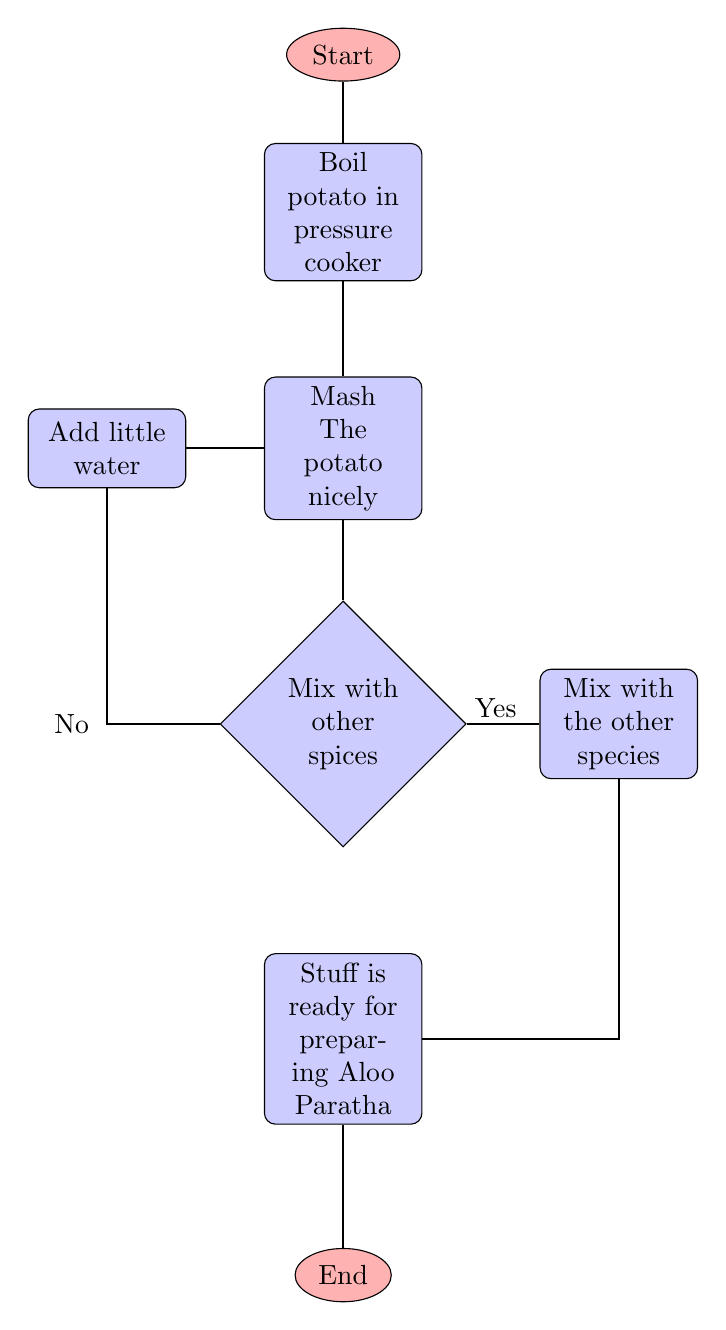
\begin{tikzpicture}[node distance=2cm]
            \node (start) [startend] {Start};
            \node (s1) [process, below of=start] {Boil potato in pressure cooker};
            \node (s2) [process, below of=s1, yshift=-1cm] {Mash The potato nicely};
            \node (s4b) [process, left of=s2,xshift=-1cm] {Add little water};
            \node (s3) [decision, below of=s2, yshift=-1.5cm] {Mix with other spices};
            \node (s4a) [process, right of=s3, xshift=1.5cm] {Mix with the other species};
            \node (s5) [process1, below of=s3, yshift=-2cm] {Stuff is ready for preparing Aloo Paratha};
            \node (end) [startend,below of=s5, yshift=-1cm] {End};
            \draw [line] (start) -- (s1);
            \draw [line] (s1) -- (s2);
            \draw [line] (s2) -- (s3);
            \draw [line] (s3) -- node[anchor=east, xshift=3mm,yshift=2mm] {Yes} (s4a);
            \draw [line] (s4b) -- (s2);
            \draw [line] (s3) -|node[anchor=west,xshift=-8mm] {No} (s4b);
            \draw [line] (s4a) |- (s5);
            \draw [line] (s5) -- (end);
            \end{tikzpicture}
            \\
            \vspace{5mm}
           Figure 1: Stuff preparation of Aloo Paratha
           \end{center}
        
        \newpage
        \section{Exotic Features}
        \subsection{Epigraph Style}
        \vspace{.5em}
        \subsection*{Chapter 1: Theory of life}
        \epigraph{\it "failure will never overtake me if my determination to succeed is strong enough."}%
         {\it og mandino}
        
        \subsection{Minipage}
        
        \begin{minipage}{0.55\linewidth}
        \begin{mdframed}
        {\emph{\LaTeX\  typesets a file of text using the TEX program and the \LaTeX\  “macro package” for TEX. That is, it processes an input file containing the text of a document with interspersed commands that describe how the text should be formatted. \LaTeX\  files are plain text that can be written in any reasonable editor. In the \LaTeX\  input file, a command name starts with a followed by either (a) a string of letters or (b) a single non-letter. Arguments contained in square brackets, [],are optional while arguments contained in braces, {}, are required.\LaTeX\  is case sensitive. Enter all commands in lower case unless explicitly directed to do otherwise.}}
        
        \end{mdframed}
        \end{minipage}
        
        \newpage
        \section{Bibliography}

    \begin{thebibliography}{} \bibitem[1]{networking} Firuza Aibara. LaTeX - Fundamental Research Group-IIT Bom- bay.http:// www.it.iitb.ac.in/frg/wiki/index.php/LaTeX/, 2016.
        \bibitem[2]{2} Leslie Lamport.{\it Latex}. Addison-Wesley, 1994.
        \bibitem[3]{3} Helmut Kopka and Patrick W Daly. A guide to latex, 1995.
        \bibitem[4]{4} Michael Downes. {\it Short math guide for LATEX.} American Mathematical Society, 2002.
    \end{thebibliography}
\end{document}
